 \documentclass[journal]{IEEEtran}
\IEEEoverridecommandlockouts
% The preceding line is only needed to identify funding in the first footnote. If that is unnecessary, please comment on it.
\usepackage{amsmath,amssymb,amsfonts}
\usepackage{algorithmic}
\usepackage{mathtools}
\usepackage{graphicx}
\usepackage{textcomp}
\usepackage{xcolor}
\usepackage{placeins}
\usepackage{minted}
\usepackage[backend=biber,style=ieee]{biblatex}
\addbibresource{sources.bib}
\def\BibTeX{{\rm B\kern-.05em{\sc i\kern-.025em b}\kern-.08em
    T\kern-.1667em\lower.7ex\hbox{E}\kern-.125emX}}

\begin{document}

\title{Geometry-Agnostic Mutual Coupling Calibration for Phased Array Radar Systems}

\author{Zachary~Sasser,~\IEEEmembership{Student Member,~IEEE,}
        Caleb~Fulton,~\IEEEmembership{Senior Member,~IEEE,}
        and~Mark~Yeary,~\IEEEmembership{Fellow,~IEEE}\\
\thanks{Zachary Sasser, Caleb Fulton, and Mark Yeary are with the School of Electrical Engineering and the Advanced Radar Research Center, University of Oklahoma, Norman, OK 73019 USA (e-mail: physics@ou.edu; fulton@ou.edu; yeary@ou.edu).}%
}

\maketitle


%%%%%%%%%%%%%%%%%%
\begin{abstract}
Phased array radar systems require precise calibration to ensure accurate beam steering and signal processing. Variations in antenna elements can significantly affect system performance, and traditional calibration methods, which rely on known geometries and specialized equipment, often struggle in real-world settings where data may be incomplete due to factors like amplifier saturation and diverse element configurations.

To overcome these limitations, we propose a geometry-agnostic calibration approach that uses mutual coupling measurements for robust calibration, independent of specific antenna configurations. By employing various computational techniques, our method supports both in-situ and initial calibration scenarios, offering flexibility for diverse radar systems, including those with non-planar or independently deployed antennas. The proposed methodology not only generalizes prior calibration techniques but also demonstrates significant improvements in calibration accuracy and operational flexibility, making it a promising solution for applications where traditional methods are impractical.
\end{abstract}

\begin{IEEEkeywords}
phased array radar, mutual coupling, calibration, partitioning, phase alignment
\end{IEEEkeywords}


%%%%%%%%%%%%%%%%%%%%%%%
%%%%%%%%%%%%%%%%%%%%%%%
\section{Introduction}
Phased array radar systems require precise calibration to ensure accurate beam steering and subsequent downstream signal processing. These radars rely on controlling the phase and amplitude of signals transmitted or received by an array of antennas. Calibration is essential for correcting variations in individual antenna elements and their associated electronics, which can lead to errors in the radar beam’s direction and shape. Without proper calibration, radar performance in detecting, tracking, and imaging targets would be compromised. A common calibration approach for stationary systems is park and probe, which involves using an external probe antenna with known characteristics to align each element \cite{simpleParkProbe,fastSimplePP,seker,brown2014phased}. This typically requires a near-field scanner large enough to accommodate the radar array. However, recent advancements in calibration algorithms allow for calibration through mutual couplings \cite{horuscal, dipole, largeScale,bekers,hassett,mitchell,fulton,aumann,dipole,embeddedFeedLineCal,javier,seker,lebron, herd2015}. In these methods, data collection involves transmitting from one element and measuring the signal received by each other element. The resulting signal is analyzed by comparing the peak of the matched filter response from the transmitted signal to the peak of the matched filter from the received signal, yielding a complex coupling coefficient. These coefficients are compiled into a coupling matrix, which is then used, along with other reference information, to compute alignment weights for each element.

Phased array calibration algorithms can be categorized based on several factors. One key distinction is whether the algorithm is intended for use in a laboratory or factory setting, where operators typically have access to specialized equipment such as near-field or far-field scanners, or a reference antenna with a known complex gain. These are referred to as ``initial calibration'' algorithms, which tend to be more precise but are often impractical for certain radar systems and cannot be applied after the radar is deployed. In contrast, ``in-situ'' calibration algorithms are designed for use with operational radar systems in the field. Another distinction is whether the algorithm depends on external equipment, such as a calibration antenna or coupled lines at each element, or whether it operates solely on the radar's internal measurements. Recent developments have focused on algorithms that do not require additional hardware, relying instead on mutual coupling measurements \cite{horuscal,dipole,largeScale,bekers,hassett,mitchell,fulton,aumann,dipole,javier,seker,lebron}.

To provide the proper framework for this paper’s technical contributions, let us first briefly survey existing mutual coupling calibration methods and discuss their limitations.  A common issue with these algorithms is their reliance on known geometry, which often requires hard-coded logic for effective implementation \cite{javier,mitchell,bekers, sasser}. This can be problematic when applying the algorithms to real-world systems, as mutual coupling data sets are often incomplete due to engineering constraints in the RF front-end design. For example, closely spaced elements can lead to amplifier saturation, causing non-linear behavior in the system \cite{MCeffects,zacharydunn,balanisant,bekers,sasser}. Although one might consider reducing transmit power to avoid saturation, this compromises the radar’s range, lowering the received signal power at more distant elements and limiting meaningful measurements. The ideal calibration algorithm should be flexible enough to account for missing data, whether due to faulty channels, missing elements, or amplifier saturation. Algorithms that depend on precise geometric knowledge often require complex logic to address such gaps.

\begin{figure*}[hptb]
    \centering
    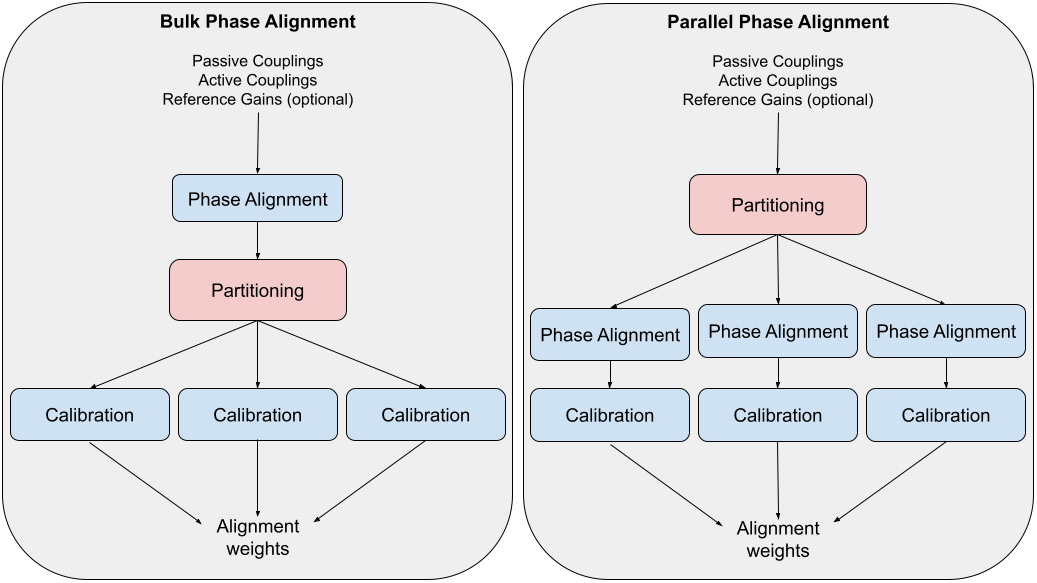
\includegraphics[width=0.8\linewidth]{orderOfOperations.png}
    \caption{Some phase alignment routines are more efficient or easier to implement when applied to a bulk dataset shown on the left. If the process can be parralelized without significant loss in quality, it is better to apply phase alignment to each subdivision after partitioning shown on the right.}
    \label{fig:orderOfOperations}
\end{figure*}

This paper proposes a geometry-agnostic calibration methodology. The approach involves three stages: partitioning, phase alignment, and a main alignment stage. Before the main calibration can be applied, a phase alignment must be performed on the data to avoid phase wrapping conditions. Partitioning is the process of subdividing the datasets into subarrays in order to parallelize the computation. Partitioning can be applied before or after phase alignment, depending on the nature of the phase alignment process being applied. Some phase alignment routines are more efficient or easier to implement when applied to a bulk dataset, such as the subtractive alignment method discussed later. If the process can be parallelized without significant loss in quality, such as in the guided phase alignment method, it is better to apply phase alignment to each subdivision after partitioning. This order of operations is depicted in Fig.~\ref{fig:orderOfOperations}

In this paper, we will outline novel geometry-agnostic techniques to achieve each stage. The proposed method is capable of calibrating antennas in arbitrary configurations, and it can also complement and extend previous mutual coupling calibration approaches. Modern tools, such as the method of moments \cite{balanisant,MCeffects} and Ansys Electronics Desktop (HFSS) \cite{HFSS}, enable the simulation of passive couplings. Instead of relying on geometric assumptions about element couplings, we propose directly evaluating the couplings based on estimates. In the case of in-situ calibration, the passive couplings are obtained through mutual coupling measurements taken after an initial calibration procedure. Importantly, when using guided approaches, the passive coupling estimates do not need to be numerically precise. These estimates only need to indicate which coupling pairs are likely to be similar. If two couplings are close after calibration, their passive estimates should be similarly close. This methodology’s flexibility allows existing calibration methods to be incorporated into a unified computational framework.

The calibration weights derived from our geometry-agnostic method are validated against reference measurements taken using our near-field setup shown in Fig.~\ref{fig:panel}. In this configuration, a near-field scanner systematically measures the complex coupling between each array element and a reference probe at fixed spacing. By comparing element responses relative to a central reference element, we obtain the precise gain and phase relationships used to verify our mutual coupling calibration results. The park-and-probe derived weights serve as the accuracy benchmark for data shown throughout this document. In a practical scenario, the starting gains would not be known until the algorithm derives alignment weights. The data shown throughout this document applies the alignment weights obtained to the gains obtained through park and probe measurements, as the method is well known to produce accurate gain estimations \cite{simpleParkProbe,fastSimplePP,seker,brown2014phased}. Before we can discuss the details of the methodology, there are practical considerations that must be discussed.

%%%%%%%%%%%%%%%%
%%%%%%%%%%%%%%%%
%\section{Practical Constraints in Mutual Coupling-Based Calibration}
\section{Overview of Calibration Methodology and Practical Constraints}


Mutual coupling-based calibration offers a compelling alternative to traditional phased array radar calibration techniques by eliminating the need for external reference equipment. These methods estimate alignment weights based solely on inter-element coupling measurements. However, when applied to real-world systems, several practical constraints must be addressed to ensure accurate and robust calibration. This section outlines the major limitations observed in experimental datasets and provides insight into their impact on calibration algorithm performance. Which constraints apply depends on the capabilities of the system in question.

%\subsection*{Measurement Saturation due to Strong Coupling}

Closely spaced radiators exhibit stronger mutual coupling, which can lead to saturation of the receiver Low Noise Amplifier (LNA) \cite{jablon}. To mitigate this, measurements that exceed the LNA’s linear operating range are clipped during acquisition, resulting in missing or unusable data entries. While adjusting the gain of the transmit and receive paths can sometimes maintain linearity, this approach is limited by the trade-offs introduced by other constraints in the system.

% \subsection*{Insufficient Coupling from Distant Elements}

At the opposite end of the coupling spectrum, radiators that are farther apart may not couple strongly enough for the signal to be detected reliably. These weak measurements often fall below the matched filter's detection threshold and are recorded as missing information, particularly when gain settings are tuned to avoid adjacent element saturation. As seen in Fig.~\ref{fig:visualizedCouplings}, this leads to a sparsely populated coupling matrix, which can hinder the construction of a fully constrained system of calibration equations.  

%\subsection*{Sub-array Isolation Limitations}

In modular systems such as the Horus polarimetric phased array radar \cite{horusgeneral,horuscal,yeary2021}, the front-end architecture is composed of Octoblades, each containing 16 ports across 8 dual-polarization channels. 
For instance, the left side of Fig.~\ref{fig:panel} depicts one 8 element x 8 element panel of Horus' multi-panel array.  While convenient for scalability, these panels suffer from limited internal channel isolation. Consequently, mutual coupling measurements between elements on the same Octoblade are censored in software to avoid contamination by cross-talk. Although hardware improvements could address this limitation, current algorithms must accommodate the resulting data gaps.  In this paper, we assume the standard $\lambda / 2$ element spacing; moreover, this is how Fig.~\ref{fig:panel} was designed by teammates in our lab.  


\begin{figure}[hptb]
    \centering
    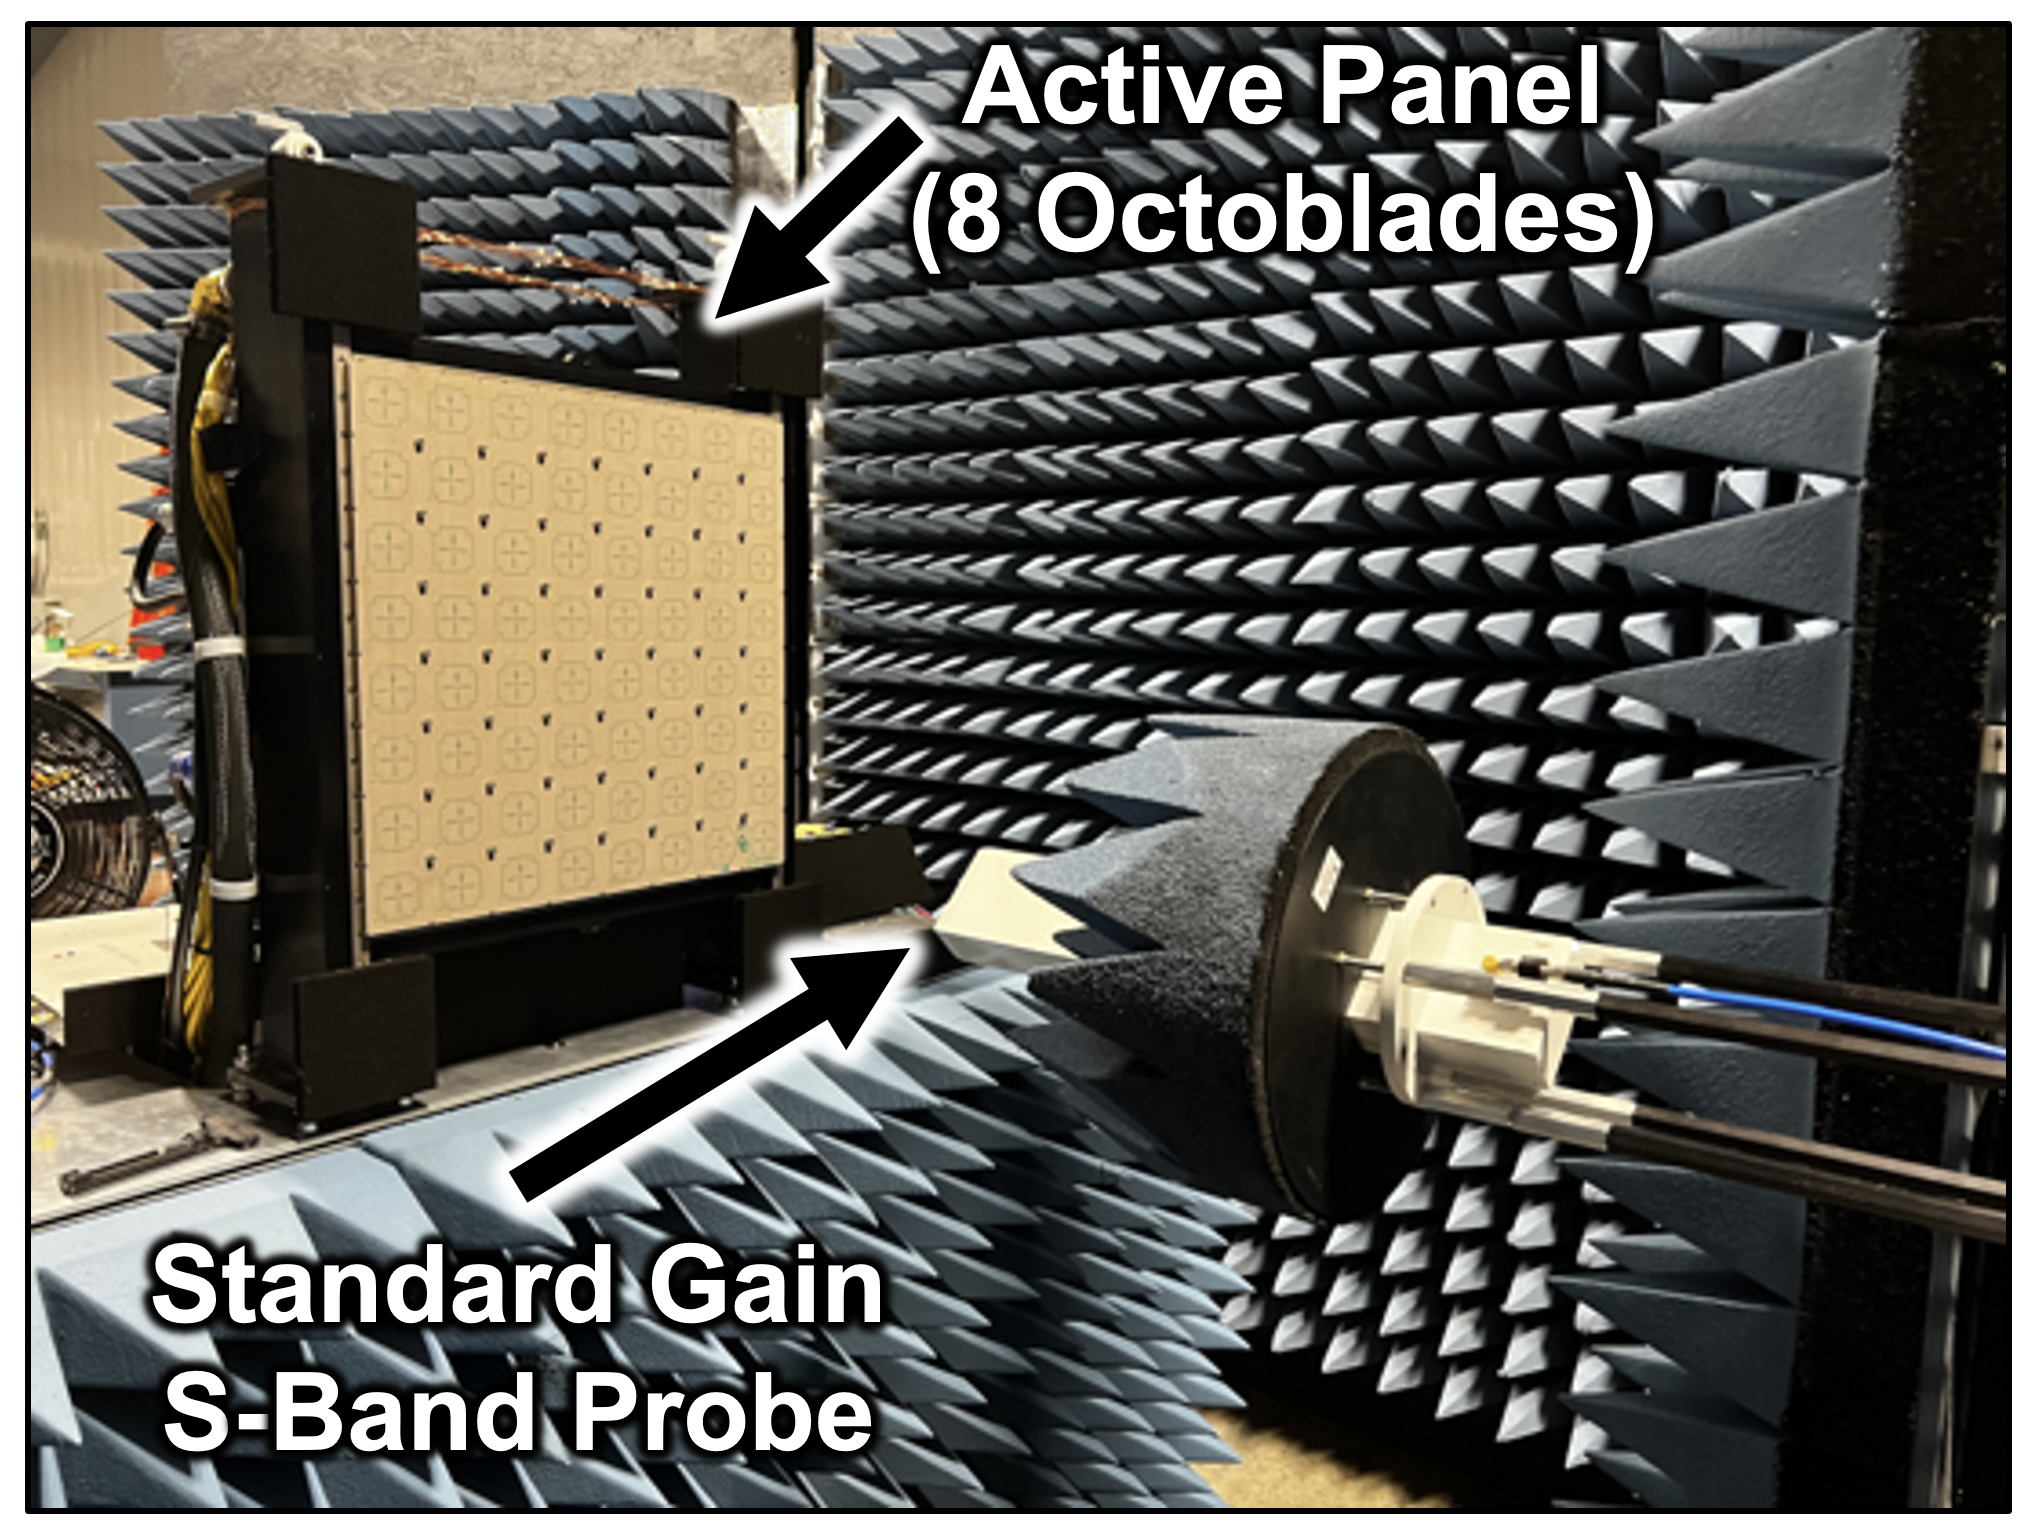
\includegraphics[width=0.9\linewidth]{panel_measurement.png}
    \caption{Configuration for park and probe measurements in our lab.}
    \label{fig:panel}
\end{figure}




%%%%%%%%%%%%%%%%
% \subsection*{Hardware Faults and Masking Strategies}

Phased array systems are susceptible to faults such as dead or missing elements and uninstalled subpanels. These issues can significantly distort the mutual coupling matrix if not properly accounted for. While faults can be detected using statistical thresholds derived from nominal system behavior \cite{lebron,diagnostic}, this method becomes ineffective when the number of faulty elements is high, leading to an under-determined system with corrupted rows and columns. In addition, there are many situations where it may be necessary to ignore certain elements and/or directions (for example when using a ``thinned array'' for receivers) \cite{nickel}. To address these concerns, masking mechanisms are implemented in the calibration pipeline to exclude affected elements from the computation. Masking can be applied at the element-direction or element-pair level, enabling, for example, receive-only exclusion of an element or suppression of specific transmitter–receiver interactions. 

\begin{figure*}[t]
    \centering
    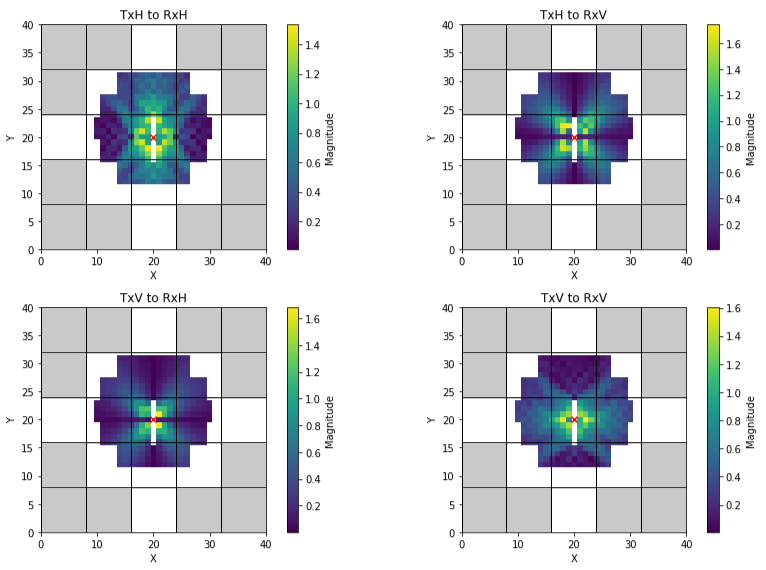
\includegraphics[width=0.92\linewidth]{visualizedCouplingsFixed.png}
    \vspace{-0.2in}
    \caption{Visual representation of coupling magnitudes in a 40x40 dual-polarized radar array. The data corresponds to all coupling measurements involving the central transmitter (denoted by a red \textbf{x}). Effects of long-range coupling limitations and sub-array censoring are visible. Black lines demarcate the modular 8x8 subpanels composing the full antenna array. The gray subpanels indicate panels which were not installed for these measurements (sub-array censoring). The white space at the end of the circle represents data that is missing due to range limitations. The white column in the center are elements which are controlled by the same Octoblade as the transmitting element. The adjacent element effects are not significant enough to warrant censoring in this case, but does result in less stable couplings near the transmitting element.}
    \label{fig:visualizedCouplings}
\end{figure*}


%%%%%%%%%%%%%%%%%%%%%%%%%
%%%%%%%%%%%%%%%%%%%%%%%%%
% \section{Coupling Model}
\subsection{Active and Passive Couplings}

%%%%%%%%%%%%%%
% \subsection*{Passive Couplings (“reference matrix”)}

\begin{figure}[hptb]
    \centering
    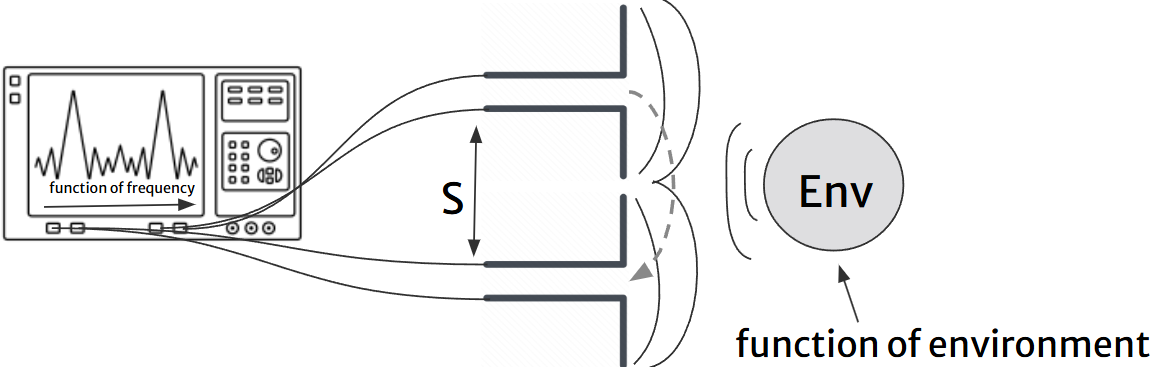
\includegraphics[width=1\linewidth]{PassiveCouplingWithArrow.png}
    \caption{An illustration to convey the dependence of passive couplings on frequency and environment.}
    \label{fig:passiveCoupling}
\end{figure}

There are two types of coupling matrices for mutual coupling calibration. First, there is the passive coupling matrix as shown in Fig.~\ref{fig:passiveCoupling}. In prior literature, this was simply referred to as the S-parameters (\cite{bekers} being a notable exception), this terminology would not be accurate in all cases. This more specific terminology allows us to avoid potential situations where S-parameters do not align with the following description. The passive coupling is a complex number that represents how the signal is changed from transmission to reception when the gains from both of the frontends are normalized to unity gain. It is assumed that only one transmitter is active at a time when the data is collected. Generally, this is intended to characterize the effects of electromagnetic transmission between the two radiators imposed on the signal as the multiplication of a complex number. It is important to note that passive coupling is a function of both frequency and environment.  Here, ``environment'' refers to the physical space of where the data were collected, such as a multi-path free anechoic chamber. 



%%%%%%%%%%%%%%
% \subsection*{Active Couplings (“measured matrix”)}

Active couplings are a function of the passive couplings and are a characterization of the total change to the signal, as depicted in Fig.~\ref{fig:ActiveCoupling}.  To begin with, the left side of Fig.~\ref{fig:ActiveCoupling} refers to the transmit portion, while the right side of the figure refers to the receive portion.  To bridge both sides, we introduce the notation $S_{ji}$ that represents electromagnetic coupling for transmitting element $i$ and receiving element $j$.  The variable $D_{ij}$ contains the {\em actual} complex coupling measurement. Next, for an array, Fig.~\ref{fig:couplingMatrix} shows an example arrangement of a coupling matrix structure that works well for us. 
%%
%%
The complex gains characterize the amplifiers and any other effects imposed on the signal by the front-end \cite{seker,lebron}. A mutual coupling measurement should be at the same frequency and in a comparable environment to that which was used for the passive coupling.

It is important to distinguish between \emph{gain factors} and \emph{alignment weights}. The complex gain factors $T_i$ and $R_j$ represent the actual, uncalibrated amplitude and phase response of the transmit and receive front-end chains, respectively. These gains encompass all linear effects imposed on the signal by amplifiers, phase shifters, and other components in the signal path. The \emph{alignment weights} are the computed correction factors applied to compensate for these gain variations. Specifically, if $T_i$ represents the complex gain of transmitter $i$, then the corresponding alignment weight $w_{T_i}$ is chosen such that $w_{T_i} \cdot T_i = 1$ (or a common complex constant across all elements). Thus, the alignment weights are essentially the multiplicative inverses of the gain factors.

The ultimate goal of calibration is to compute these gain factors so alignment weights can be applied to the amplifiers aligning each radiator in magnitude and phase. In the best-case scenario, the calibrated gains would be unity, however in many cases it is acceptable as long as all the gains are equal. If the system is linearized, the alignment weights should map the passive coupling matrix to the active coupling matrix.
%%
%%
The next subsection builds on this theme to construct a set of linear equations that are solvable for the calibration solution. 


\begin{figure}[hptb]
    \centering
    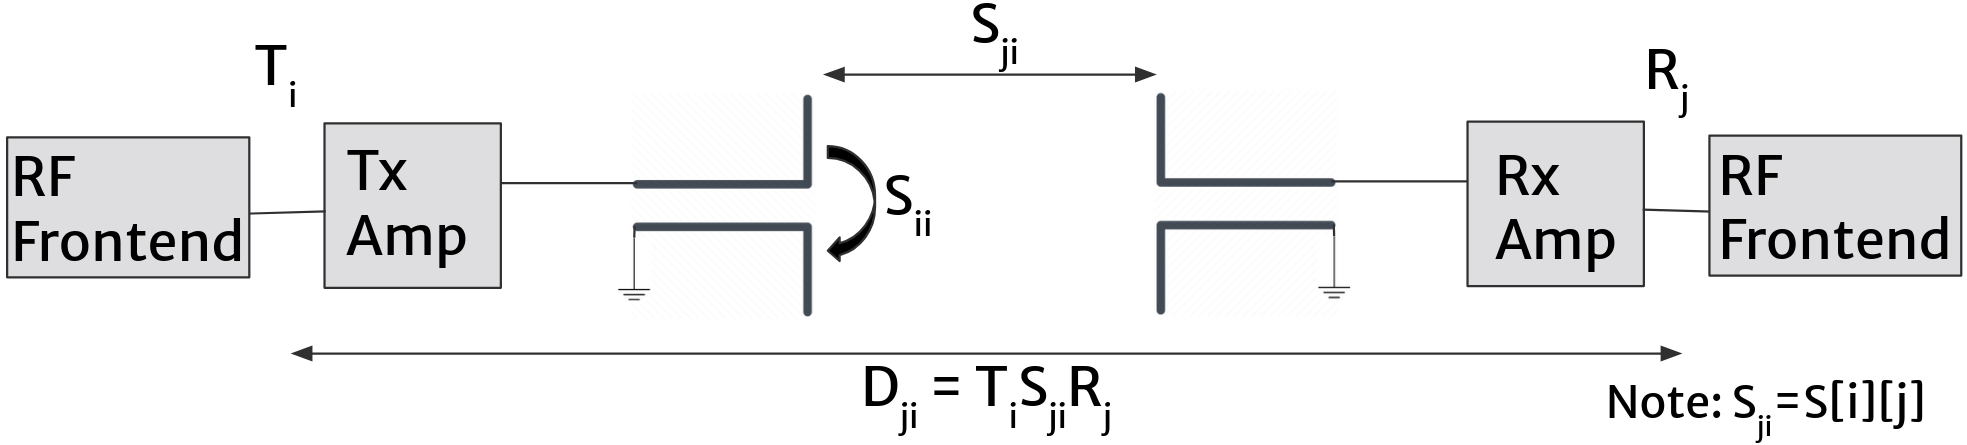
\includegraphics[width=1\linewidth]{ActiveCoupling.png}
    \vspace{-0.2in}
    \caption{A signal path block diagram illustrating that active couplings are directly related to the passive couplings but include the effects introduced by the front-end representing the overall effect with a complex value known as a gain for transmit and receive.}
    \label{fig:ActiveCoupling}
\end{figure}

\begin{figure}[hptb]
    \centering
    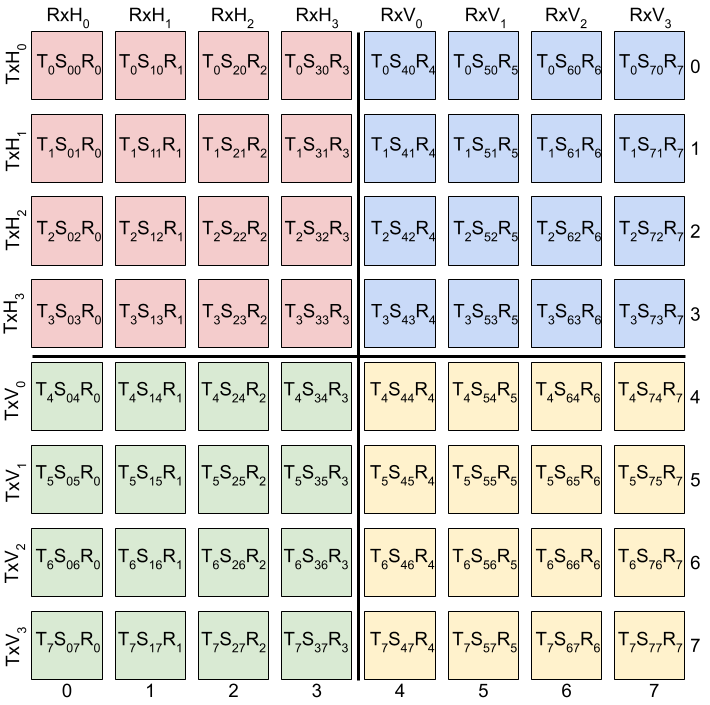
\includegraphics[width=1\linewidth]{CouplingMatrix.png}
    \vspace{-0.2in}
    \caption{A visual depiction of the coupling matrix structure used. The model shown is a hypothetical 4-element (8 radiators, 16 gains) dual-pol antenna configuration. For example, row 4 column 2 of the matrix represents transmitting from the vertical radiator of element 0 to the horizontal radiator of element 2.}
    \label{fig:couplingMatrix}
\end{figure}

%%%%%%%%%%%%%



%%%%%%%%%%%%%%
\subsection{Coupling Model}

The calibration process begins with an uncalibrated coupling matrix $\mathbf{D} \in \mathbb{C}^{N \times N}$, where $N$ represents the total number of radiators (including both polarizations for dual-pol systems). Each entry $D_{ij}$ contains the complex coupling measurement between transmitter $i$ and receiver $j$, formed as the product
%%
%%
$D_{ij} = T_i S_{ji} R_j$,
%%
%%
% \begin{equation}
% D_{ij} = T_i S_{ji} R_j ~~, 
% \end{equation}
%%
%%
%\noindent 
where $T_i$ and $R_j$ are the unknown complex gains of the transmit and receive chains respectively, and $S_{ji}$ represents the passive coupling between radiators. For an $N$-element system, $\mathbf{D}$ exhibits block structure when accounting for polarization diversity, as illustrated in Fig.~\ref{fig:couplingMatrix}. The calibration problem reduces to estimating $T_i$ and $R_j$ given $\mathbf{D}$ and an estimate of the passive couplings $\mathbf{S}$. From $\mathbf{D}$, we compute ratios $K^{a,b}_{c,d} = D_{a,b}/D_{c,d}$ as shown in \eqref{eq:Kfull} as

\begin{equation} \label{eq:Kfull}
    K^{a,b}_{c,d} = \frac{D_{a,b}}{D_{c,d}} = \frac{T_aS_{b,a}R_b}{T_cS_{d,c}R_d} ~~. 
\end{equation}

However, due to the large number of unknowns in this expression, solving a complete system based solely on this formulation is not feasible. To reduce the problem to a tractable form, we impose a constraint on the system by only considering cases where the passive coupling terms are approximately equal: \( S_{b,a} \approx S_{d,c} \). This assumption reduces the system to a lower-dimensional vector space, making it possible to determine the solution. The simplified expression is shown in equation \eqref{eq:Kred} \cite{fulton,mitchell} and expressed as

\begin{equation} \label{eq:Kred}
    S_{b,a} \approx S_{d,c} \implies K^{a,b}_{c,d} = \frac{D_{a,b}}{D_{c,d}} = \frac{T_aR_b}{T_cR_d} ~~.
\end{equation}


\noindent 
This product-based relationship is not compatible with linear algebraic methods. To apply matrix-based techniques, we take the logarithm of both sides, converting the multiplicative relationship into an additive one, as shown in equations \eqref{eq:ln1} and \eqref{eq:ln2}. The base of the logarithm is flexible, and base 2 is commonly used due to its favorable dynamic range and compression properties \cite{javier}.

\begin{subequations}
\begin{equation}\label{eq:ln1}
    \log\left(\frac{D_{a,b}}{D_{c,d}}\right) = \log\left(\frac{T_a R_b}{T_c R_d}\right)
\end{equation}
\begin{equation}\label{eq:ln2}
    \begin{aligned}
        \implies \log(D_{a,b}) - \log(D_{c,d}) &= \log(T_a) + \log(R_b) \\
        &\quad - \log(T_c) - \log(R_d)
    \end{aligned}
\end{equation}
\end{subequations}

We now define a vector \( \vec{\mathbf{E}} \), which contains the logarithmic values of all unknown gains—both transmit and receive. Each equation in the system can be represented by a row in a matrix \( \bar{\mathbf{A}} \), with entries existing in the set \{-1, 0, 1\} indicating the role of each gain in that equation. The resulting system is expressed as

\begin{equation}\label{eq:vectorized}
    \vec{\mathbf{K}} = \bar{\mathbf{A}} \cdot \vec{\mathbf{E}} \iff \vec{\mathbf{E}} = \bar{\mathbf{A}}^{+} \vec{\mathbf{K}} ~~,
\end{equation}

\noindent 
where \( \bar{\mathbf{A}}^{+} \) denotes the Moore-Penrose pseudo-inverse. The Moore-Penrose pseudo-inverse provides a least-squares solution that exists for any matrix $\bar{\mathbf{A}}$, regardless of dimension or rank. However, for the solution to be physically meaningful and well-constrained, the system must form a connected graph where each radiator relates to at least one other radiator through valid coupling measurements. In practice, this requires that the measurement set provides sufficient independent equations to resolve all unknown gains relative to the reference elements.
Since mutual coupling measurements alone are typically insufficient to fully constrain the system, it is necessary to incorporate a-priori knowledge of at least one transmit and one receive gain. To integrate these known values, we partition the gain vector and matrix into known and unknown components. The known gain values form a vector \( \vec{\mathbf{E_2}} \) and their associated matrix columns form \( \bar{\mathbf{B}} \). The unknowns form \( \vec{\mathbf{E_1}} \) and \( \bar{\mathbf{G}} \), respectively. The resulting system is:

\begin{equation}\label{eq:vectorizedFull}
    \vec{\mathbf{K}} = \bar{\mathbf{G}} \cdot \vec{\mathbf{E_1}} + \bar{\mathbf{B}} \cdot \vec{\mathbf{E_2}} 
    \iff 
    \vec{\mathbf{E_1}} = \bar{\mathbf{G}}^{+} \cdot (\vec{\mathbf{K}} - \bar{\mathbf{B}} \cdot \vec{\mathbf{E_2}}) ~~. 
\end{equation}

A representative example of this system is shown below, illustrating how specific gain terms map into the matrix representation:

\begin{equation}
\begin{aligned}[b]
    \begin{bmatrix}
        1 & -1 & 0 & 0 & 0 & -1
    \end{bmatrix}
    & \begin{bmatrix}
        \log(T_a) \\ \log(T_c) \\ \log(T_d) \\
        \log(R_a) \\ \log(R_c) \\ \log(R_d)
    \end{bmatrix}
    + 
    \begin{bmatrix}
        0 & 1
    \end{bmatrix}
    \begin{bmatrix}
        \log(T_b) \\ \log(R_b)
    \end{bmatrix} \\  \\
    & = \begin{bmatrix}
        \log(D_{a,b}) - \log(D_{c,d})
    \end{bmatrix}
\end{aligned}
\label{Matrix}
\end{equation}

%%%%%%%%%%%%%%%%%%%%%%%%%%%
\subsection{Coupling Sets}
Coupling sets provide a systematic framework for grouping antenna pairings that are presumed to have equal passive couplings based on geometric similarity and polarization characteristics \cite{lebron,bekers,javier}. This methodology capitalizes on the electromagnetic principle that identical relative positioning and polarization states should theoretically yield equivalent coupling behavior. The approach proves particularly effective for uniformly spaced planar arrays where geometric patterns can be systematically enumerated and where boundary effects are minimized in central array regions.
%%
%%
The implementation of coupling sets offers several computational advantages. By establishing predefined grouping rules, the calibration process can be automated through straightforward indexing operations, significantly reducing the manual effort required for equation formulation. However, this convenience comes with several substantive limitations that impact calibration accuracy:

First, the fundamental assumption of geometric equivalence often fails to capture the complete set of pairings with truly identical couplings. The method inherently misses potential correlations between pairings that may exist across different geometric groups due to higher-order electromagnetic interactions or structural symmetries not captured by simple geometric rules. This interconnectivity between nominally distinct coupling sets represents valuable calibration information that is systematically excluded by the coupling set approach.

Second, practical array imperfections frequently violate the coupling equality assumption within sets. Boundary effects at array edges, manufacturing tolerances, and subtle variations in element performance introduce significant coupling variations within nominally identical geometric groups \cite{javier,lebron,bekers,diagnostic,sasser}.

Third, the indexing logic becomes increasingly complex when dealing with real-world arrays containing failed elements or non-standard configurations. The algorithm must incorporate extensive exception handling to address missing data cases, and this complexity grows combinatorially with array size and the number of allowed geometric transformations.

To mitigate these limitations, one can implement statistical filtering of coupling sets \cite{bekers}. Each candidate set is evaluated using multiple metrics: standard deviation, maximum coupling magnitude, and minimum coupling magnitude thresholds are generally adequate. Sets failing these criteria are excluded from the calibration process. The exact thresholds are highly dependent on the system in question. While this filtering improves result quality, it necessarily reduces the number of usable equations, potentially leading to underdetermined systems if applied too aggressively.
%%
%%
The effectiveness of coupling sets depends critically on the array's regularity. For non-planar arrays or systems with irregular spacing, the geometric grouping rules become either prohibitively complex or fundamentally inadequate. In this paper we will address these limitations and propose algorithms which mitigate these problems through a more dynamic approach. However, before we can apply any calibration technique, a pre-phasing stage must be performed \cite{bekers,javier,sasser} as will be described in the next section.




 

%%%%%%%%%%%%%%%
%%%%%%%%%%%%%%%
\section{Pre-alignment Considerations}

This section discusses two pre-alignment techniques, which establish a critical foundation for subsequent calibration procedures. However, they represent only the first stage in achieving full system alignment. The following sections will build upon this foundation to develop comprehensive calibration solutions that address both magnitude and phase alignment while accommodating real-world measurement constraints.



%%%%%%%%%%%%%%%
%\subsection{Phase Wrapping Mitigation}
Before applying calibration algorithms, it is essential to address phase wrapping in the measurement data. As discussed in \cite{bekers,javier,sasser}, the logarithmic transformation used in the calibration framework requires that phase variations of transmit (Tx) and receive (Rx) gains remain within $\pm 90^\circ$ to avoid ambiguity. To satisfy this constraint, we implement a preliminary phase alignment procedure that corrects for phase wrapping effects. The final calibration weights will be the product of these pre-alignment weights and those determined by the subsequent calibration process.
%%
%%
While this pre-phasing step can sometimes achieve complete phase alignment, its primary purpose is to establish a suitable initial state for the main calibration algorithm. The process is particularly crucial for systems with significant initial phase variations, though perfect alignment is not strictly required for successful calibration.


With the above concepts in mind, a logical first attempt at a geometry-independent method uses only an estimated passive coupling matrix to determine alignment weights. The process shown in Fig.~\ref{fig:PAflowchart} involves:

\begin{enumerate}
    \item[a.] Converting active and passive coupling matrices to phase representations
    \item[b.] Subtracting passive coupling phases from measured phases
    \item[c.] Referencing all phases to a chosen element
    \item[d.] Applying modulo $360^\circ$ to eliminate wrapping artifacts
    \item[e.] Computing mean phase offsets for each element
\end{enumerate}

\begin{figure}[ht]
    \centering
    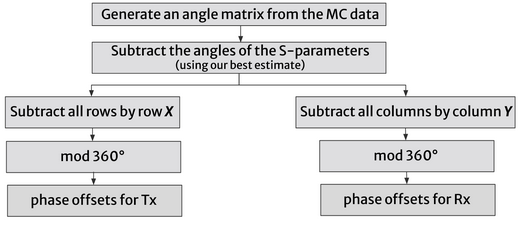
\includegraphics[width=0.95\linewidth]{phaseAlignFlowchart.png}
    \caption{Block diagram depicting steps involved in geometry agnostic phase alignment.}
    \label{fig:PAflowchart}
\end{figure}

\begin{figure}
    \centering
    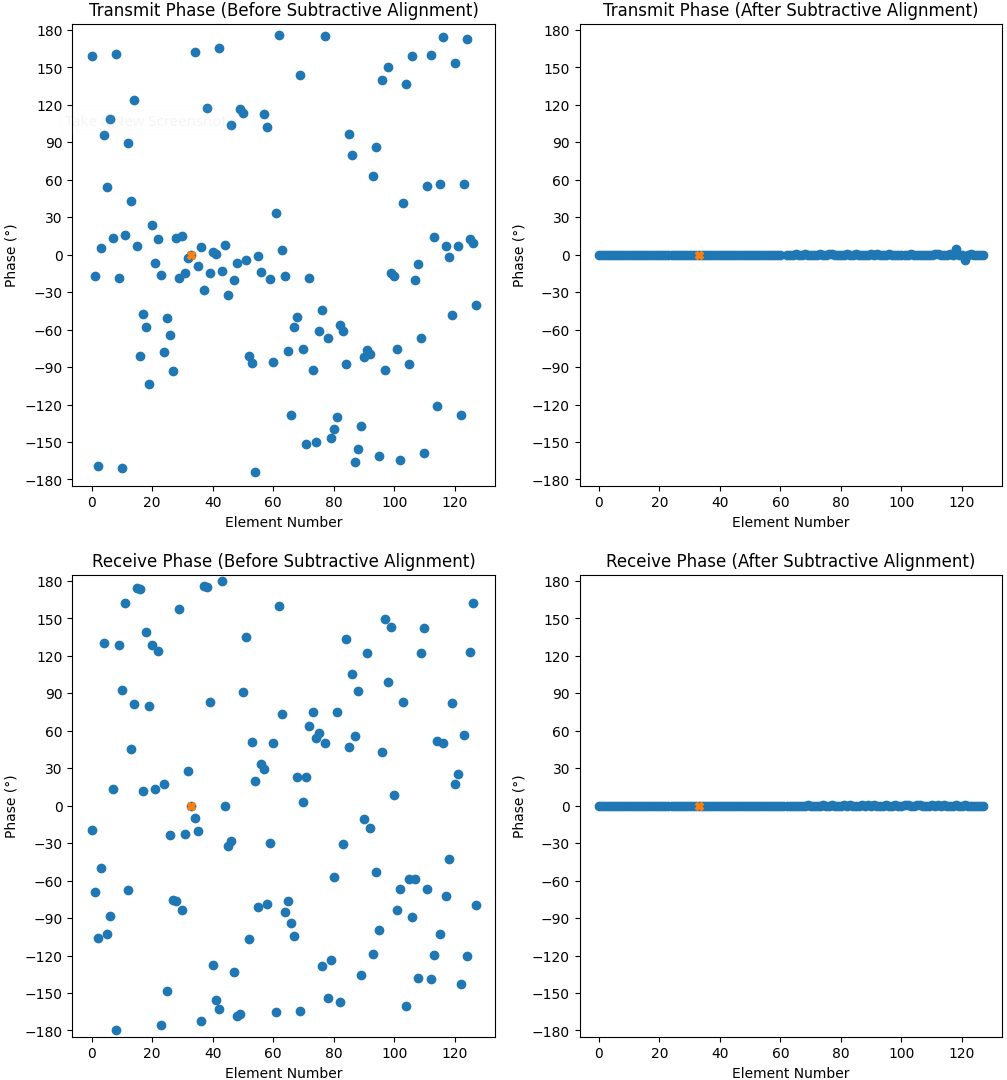
\includegraphics[width=0.95\linewidth]{subtraction-dualpole.png}
    \caption{The result of subtractive phase alignment applied to a dataset gathered on a dual-pol 8x8 system. The element marked in orange is the reference element. Phases are depicted relative to the reference element.}
    \label{fig:subtractResults}
\end{figure}

This method effectively aligns phases while avoiding geometric assumptions. However, its accuracy depends heavily on the quality of the passive coupling estimates. Any deviation from what the coupling data would be if the system were calibrated will contribute directly to errors in the results. Fig.~\ref{fig:subtractResults} demonstrates the resulting gain phases after the subtractive method is applied. In this case, the passive couplings used were highly accurate. To further improve accuracy and robustness, it is necessary to isolate the estimated dataset from the computation itself. This will reduce the sensitivity to errors in the estimated dataset. In the next section, we will describe such an algorithm. 

\begin{figure}
    \centering
    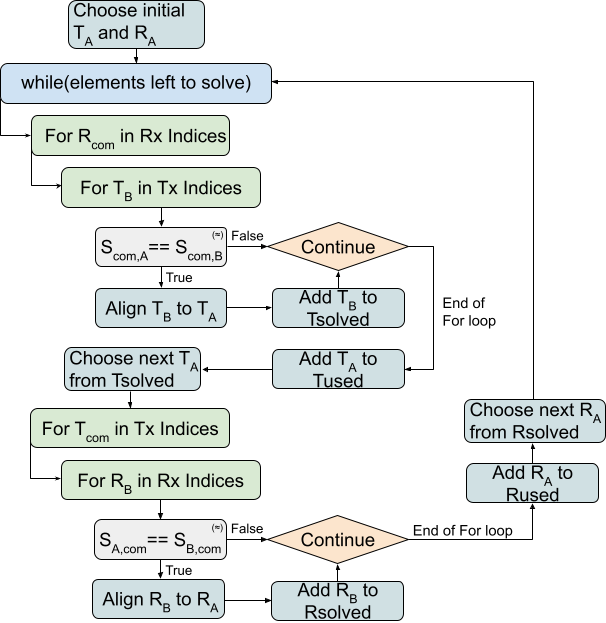
\includegraphics[width=0.95\linewidth]{Agnostic Alignment.png}
    \caption{A flowchart depicting the stages of the passive coupling guided approach to phase alignment.}
    \label{fig:agnosticPA}
\end{figure}

\noindent
{\em Guided Alignment:}
To balance accuracy and flexibility, a guided approach (Fig.~\ref{fig:agnosticPA}) is proposed that uses passive coupling estimates to identify suitable element pairings without direct geometric assumptions. In this method, initial references, $T_A$ and $R_A$, are chosen before execution. The system then loops through every combination of a common receiver ($R_{com}$) and transmitter ($T_B$) and decides if $S_{A,com}$ is close enough to $S_{B,com}$ to apply equation (\ref{eq:phaseAlign}).

\begin{align}
    S_{com,A} \approx S_{com,B} &\implies \nonumber \\
    \angle K^{com,B}_{com,A} &= \angle \frac{T_{B} S_{com,B} R_{com}}{T_{A} S_{com,A} R_{com}} = \angle \frac{T_B}{T_A} \nonumber \\
    &= \angle T_B - \angle T_A
    \label{eq:phaseAlign}
\end{align}


After element $T_B$ is aligned to element $T_A$, it is added to a list of solved elements. When all possible combinations for element $T_A$ have been enumerated, it is added to a list of used references to avoid reusing it in future loops. Then, a new $T_A$ is chosen from the list of solved elements for the next loop. The list is sorted so that the next chosen element will be the least recently solved element in order to minimize the degrees of connection to the original reference. This process is then repeated for receive. This full cycle is looped until there are no more elements to solve.

Fig.~\ref{fig:bruteforcePA} demonstrates the results of the guided phase alignment method. The algorithm's effectiveness stems from leveraging electromagnetic relationships encoded in the passive coupling matrix rather than explicit geometric rules. Instead of directly involving the passive couplings in the calculation, the coupling estimations are used as a guide to decide which pairings to apply together. In this case, the passive coupling estimate does not need to be a numerically accurate prediction of couplings taken in a calibrated state. Instead, couplings that are considered to be approximately equal in the passive coupling matrix should also be approximately equal in the calibrated measurement. While not ideal for accuracy, the algorithm would allow for assigning pairings into groups, and the passive coupling matrix would simply be composed of integers representing the group assignments. This would effectively be the same as creating coupling sets. Next, we explore the coupling linearization constraint.


\begin{figure}
    \centering
    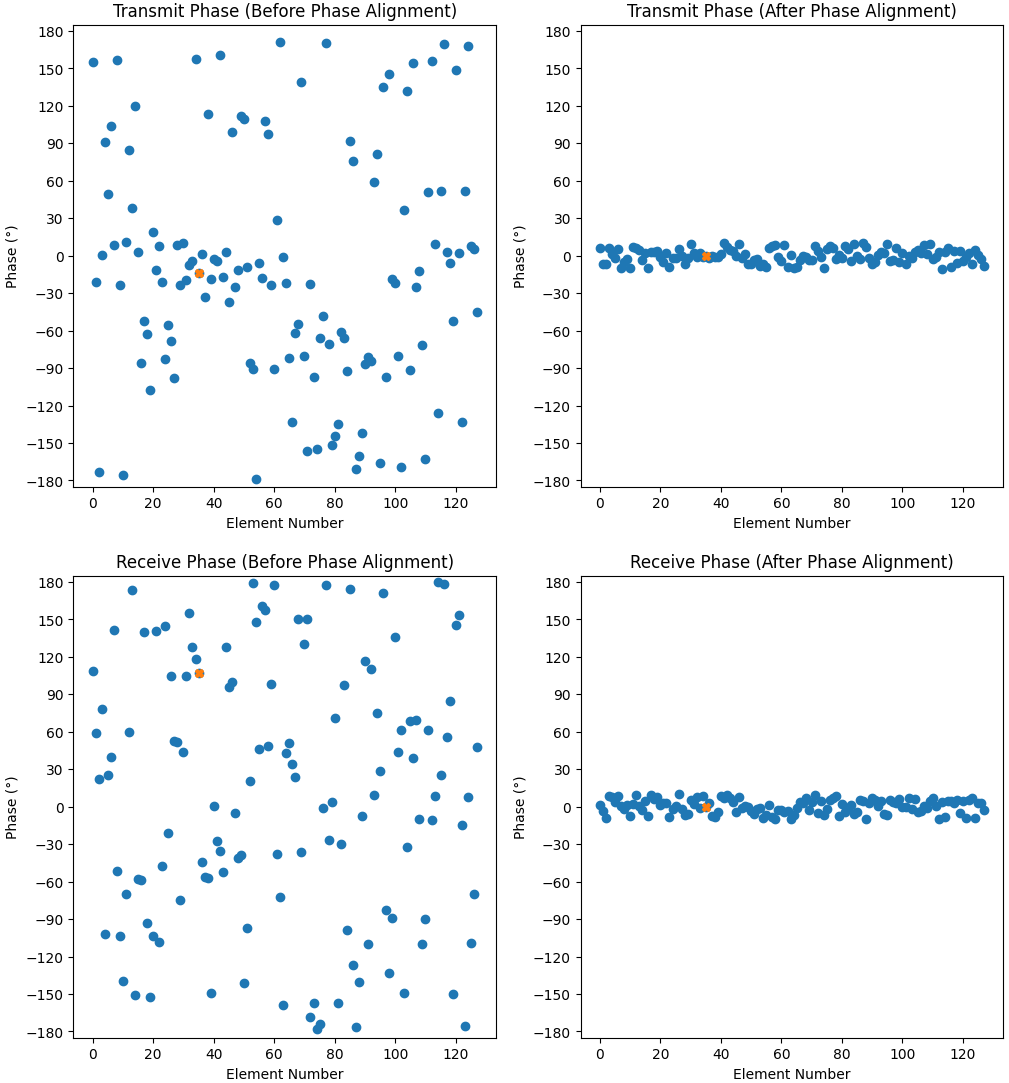
\includegraphics[width=1\linewidth]{bruteForcePAresults-dualpole.png}
    \caption{The result of guided phase alignment applied to a dataset gathered on a dual-pol 8x8 phased array system. The element used as the first reference is marked in orange. Phases are depicted relative to the reference element.}
    \label{fig:bruteforcePA}
\end{figure}



%%%% Linearization
\section{Coupling Linearization}

\begin{figure*}[ht] %figure star will span the figure over two columns 
    \centering
    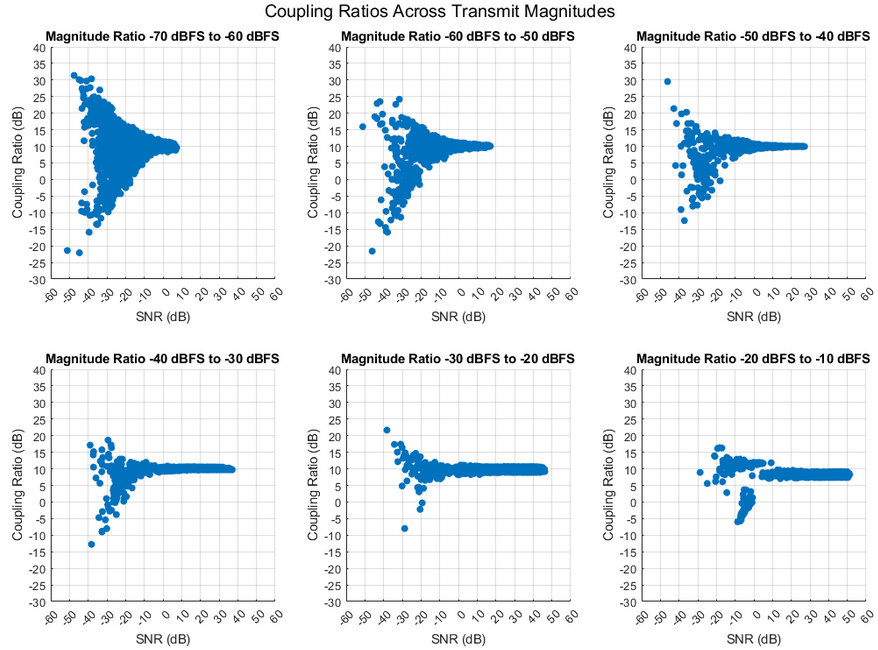
\includegraphics[width=1\linewidth]{magDiffSweep.png}
    \vspace{-0.2in} %remove space between figure and caption
    \caption{The comparison of coupling data measured across various ranges of transmit power levels.}
    \label{fig:magDiffSweep}
\end{figure*}

\begin{figure}[hptb]
    \centering
    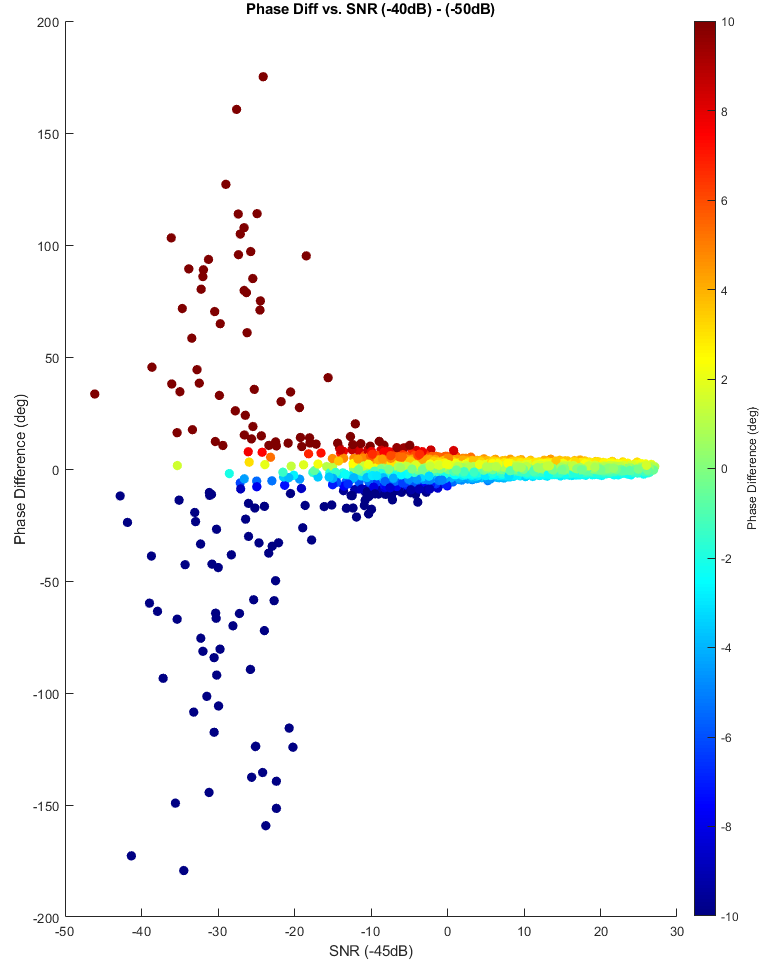
\includegraphics[width=1\linewidth]{phaseDiff.png}
    \vspace{-0.2in}
    \caption{The difference in phase between coupling data taken when the radar was set to a transmit power level of -40 dB compared to -50 dB. }
    \label{fig:phaseDiffzoomout}
\end{figure}

% \begin{figure}[hptb]
%     \centering
%     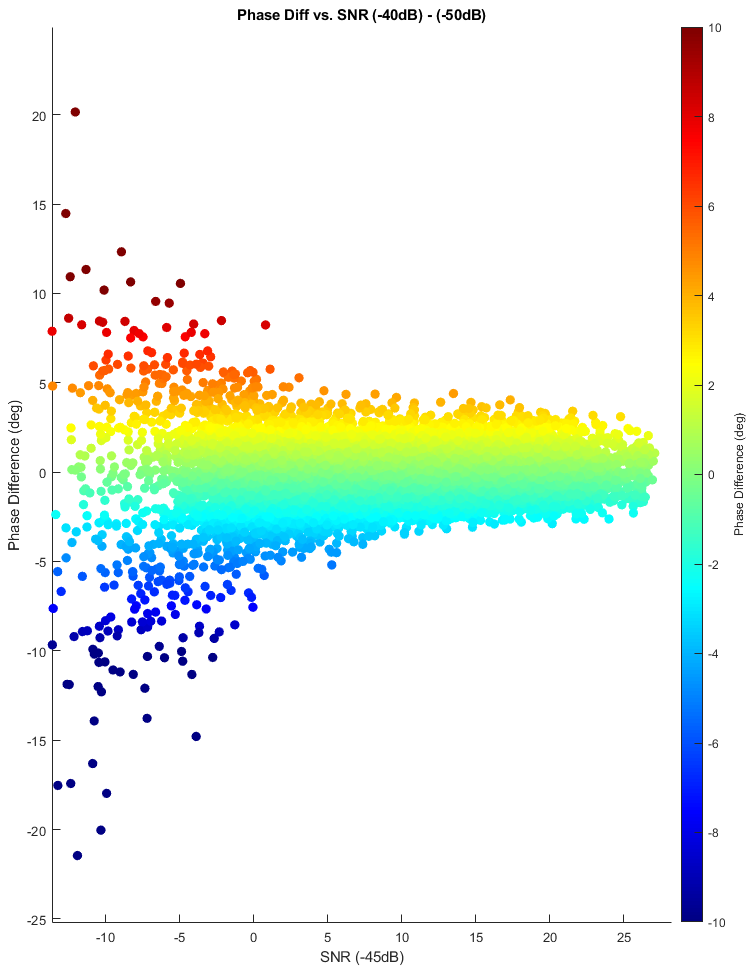
\includegraphics[width=0.8\linewidth]{phaseDiffZoomed.png}
%     \vspace{-0.1in}
%     \caption{The difference in phase between coupling data taken when the radar was set to a transmit power level of -40 dB compared to -50 dB.  Here, the plot has been zoomed in to show the high SNR measurements.}
%     \label{fig:phaseDiffcloseup}
% \end{figure}

The calibration methodologies presented in this work rely fundamentally on the assumption that the radar system operates in a linear regime. This linearity ensures that changes in transmit power produce proportional changes in received coupling measurements. In practical systems, however, nonlinear effects from amplifier saturation and noise can violate this assumption, necessitating careful system linearization before calibration \cite{sasser}.

For the calibration framework to be valid, the system must satisfy two key conditions:
\begin{enumerate}
    \item \textbf{Magnitude Linearity}: A $\Delta$ dB change in transmit power should produce a $\Delta$ dB change in all coupling measurements
    \item \textbf{Phase Stability}: Changes in transmit power should not introduce phase variations in coupling measurements
\end{enumerate}

For instance, Fig.~\ref{fig:magDiffSweep} demonstrates typical nonlinear effects observed in experimental systems. At low power levels, signal-to-noise ratio (SNR) degradation causes random magnitude variations, while high power levels drive amplifiers into saturation. Both effects violate the linearity assumptions required for calibration. To solve this problem, we have developed a gain sweep method:

\begin{enumerate}
    \item Measure coupling matrices across a range of transmit power levels
    \item Identify the linear region where magnitude changes are proportional 
    \item Verify phase stability
    \item Select operating points maintaining adequate SNR while avoiding saturation
\end{enumerate}

The effectiveness of the proposed calibration framework is inherently dependent on maintaining adequate signal-to-noise ratio (SNR) in the mutual coupling measurements. As SNR decreases, both magnitude linearity and phase stability degrade, introducing random variations that violate the fundamental assumptions of the calibration model. While the gain sweep method identifies optimal operating points that balance SNR requirements with linearity constraints, practical systems must maintain sufficient SNR to ensure reliable calibration performance. In scenarios where no linear operating region exists due to pervasive low SNR conditions, alternative calibration approaches or hardware modifications may be necessary, as the multiplicative complex gain model becomes invalid when measurement noise dominates the signal characteristics.

\noindent 
This empirical approach provides reliable linearization for many practical systems. The method is particularly effective when receive gains are digitally controlled, simplifying the optimization to a single dimension. 
%%
%%
For example, with respect to Step (2) of the method, in our case the optimal
power setting was found to be around -40 dB to -50 dB as can be
seen in Fig.~\ref{fig:magDiffSweep}. 
%%
%%
Following Step (3), Fig.~\ref{fig:phaseDiffzoomout} depicts the difference in phase between coupling data at transmit power levels of -40dB and -50dB.
As observed, the change in gain magnitude had minimal effect on the phase of the couplings as long as the SNR of the measurement was high.
%%
%%
In summary, proper linearization ensures the validity of the subsequent calibration steps while maximizing the system’s dynamic range. The next section discusses the main step of the calibration process. 



%%%%%%%%%%
%%%%%%%%%%%
\section{Main Alignment Stage}
The proposed calibration framework employs an object-oriented approach to manage the system of equations required for calibration. Key system attributes, including the number of elements and the coefficient matrix $\bar{\mathbf{A}}$, are encapsulated within a computational class structure. This design maintains metadata about equation pairings to facilitate efficient updates to the measurement vector $\vec{\mathbf{K}}$ without matrix reconstruction. Notably, the implementation does not distinguish by element but instead by radiator. For human accessibility, the vertical polarization is placed directly after the horizontal for indexing purposes. However, the algorithm itself treats every radiator index as an arbitrary independent antenna. The framework implements a filter at the point of insertion into the system of equations. Whenever a pairing is requested to be added to the system, the function checks for various conditions such as whether the pairings involved exist in the dataset, if the passive coupling values are close enough for inclusion, if the SNR is high enough to be considered valid, and any other checks the system requires to determine validity of an equation. If the pairing requested passes the filter checks, the system adds the entry to the system of equations; otherwise, the function simply returns 0, effectively rejecting the pairing \cite{sasser}. 

It is important to clarify that the rejection operates at the equation level rather than at the level of individual pairings. Each equation consists of two pairings, one contributing +1 matrix entries and one contributing -1 entries such that a rejected equation may still be represented elsewhere in the system through an alternative valid combination. As such, there is no fixed rejection percentage beyond which the calibration becomes unsolvable; solvability depends not on the raw number of accepted equations, but on whether the remaining equations form a sufficiently connected graph across all radiators. In practice, as long as each radiator maintains multiple independent valid connections to the network, the least-squares system remains well-posed. However, if filtering becomes so aggressive that large subsets of radiators are never related through any admissible equation, the solution will naturally become underdetermined.

This architecture provides two key advantages:

\begin{enumerate}
    \item \textbf{Decoupled Estimation}: Passive coupling estimates guide equation formation without directly entering computations, reducing sensitivity to estimation errors
    \item \textbf{Modular Filtering}: Validation criteria are applied at the point of measurement insertion, simplifying higher-level algorithm implementation
\end{enumerate}


The most exhaustive approach evaluates all possible radiator combinations ($O(N^4)$ complexity), offering complete system characterization. While this may not be the most computationally efficient algorithm, it does tend to produce solutions in a reasonable amount of time, so long as the array it is being applied to is of reasonable size. This approach is advantageous over previous coupling set-based methods for two reasons. First, forming couplings into groups introduces the possibility for couplings that may have made valid pairings to be excluded simply because they were placed in different groups. A subset of group A might pair with a subset of group B, but because these groupings were used, certain interconnections would not be considered. Second, often when couplings are lumped into groups (ex. based on relative geometry), it is assumed that all of the couplings within that group are close enough to be paired. However, this condition is often violated, especially as the group sizes become larger. For example, if using relative geometry, element pairings that are closer to the edge will experience edge effects and may not be comparable to a coupling of similar spacing in the center of the array \cite{javier,lebron,bekers,diagnostic,linder2025sub,sasser}. In practice, the way this error is mitigated is by statistical rejection of sets (ex. standard deviation). With the introduction of this method, all possible valid equations are included while systematically avoiding equations that violate the desired metrics. 


\begin{figure}
    \centering
    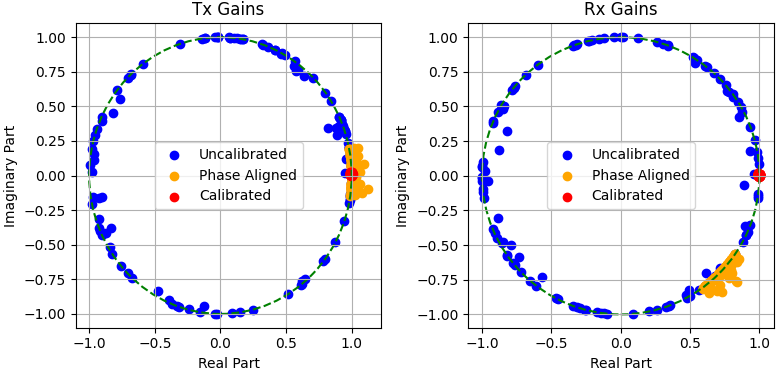
\includegraphics[width=1\linewidth]{guidedResults-dualpole.png}
    \caption{The result of guided phase alignment applied to a dataset gathered on a dual-pol 8x8 phased array system (64 elements, 128 radiators, 256 gains). Blue: The ground truth gains obtained by inverting the alignment weights obtained through park and probe. Orange: After guided phase alignment correction is applied. Red: After phase correction and alignment weights have been applied. There are 128 data points of each color in both plots, and many data points overlap.}
    \label{fig:guidedResults}
\end{figure}

Fig.~\ref{fig:guidedResults} demonstrates the results of the brute-force alignment process. The gains of the radiators begin in random starting states indicated in blue. The guided pre-alignment process is then applied, resulting in the phase-aligned gains shown in orange. Finally, the main brute-force alignment process is applied which aligns all 128 radiators to unity gain.

If the reference gain information is not provided, the system of equations will always be circularly defined. It is possible to obtain relative gains without a reference, which can be useful depending on how alignment weights are applied in the frontend systems. In the cases where a reference gain cannot be provided, every radiator can be aligned to a reference radiator by setting the gain of the reference to one in the computation. For many applications, this relative alignment may be adequate. Effectively, this defines unity gain to be in reference to the state of that particular radiator. The error will manifest as a signal delay, but one that is constant across all elements since they are aligned with each other. An example of this alignment applied to a phased array system is shown in Fig.~\ref{fig:unityRefGains}.


\begin{figure}[hptb]
    \centering
    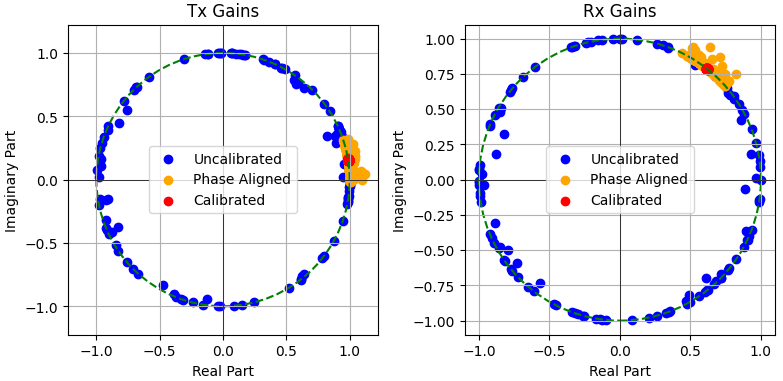
\includegraphics[width=0.98\linewidth]{refGain2.png}
    \caption{The result of calibration performed on data from a dual-pol 8x8 system if the reference gains are assumed to be unity. All elements are aligned to the complex gain of the reference element.}
    \label{fig:unityRefGains}
\end{figure}





%%%%%%%%%%%%%%%%%%
%%%%%%%%%%%%%%%%%%
\section{Partitioning Strategies for Large Arrays}

For large arrays, it is often impractical to perform the calibration computations in a reasonable amount of time, given approximately $N^4$ number of operations for $N$ elements.
For this reason, it is necessary to subdivide the array into partitions that can be solved independently. The next two sub-sections describe our approaches to solving this problem.





%%%%%%%%%%%%%
\subsection{Panel Subdivision Method}

For large regular arrays, the panel subdivision approach divides the system into modular panels, as depicted in Fig.~\ref{fig:panelSubdivision} \cite{sasser}.
%%
%%
Here, each individual element is shown as a small colored box. Elements that are solved or provided as a-priori are shown in blue. Elements that are solved in that step are shown in green. Red indicates elements that are unsolved. 
%
The left half of Fig.~\ref{fig:panelSubdivision} shows the first stage, where the starting reference is used to align a center element in each of the subdivisions. This effectively creates a reference element that can be used for each subdivision.
%
The right half of Fig.~\ref{fig:panelSubdivision} shows one subdivision being solved utilizing one of the references computed in the previous step.
%%
%%
Many radar systems use independent modular panels and/or sub-array processing, with each sub-array having a prescribed set of elements; therefore, a panel subdivision approach is a natural outcome of modern phased array data processing techniques \cite{horuscal,horusgeneral,benefits,linder2025sub,ganti2018calibration,brown2014phased,pesavento2002direction, nickel,conway2018, harger2021, conway2013, herd2015}. In summary, the method proceeds as follows:
%%
%%
\begin{enumerate}
    \item \textbf{Reference Selection}: Designate reference elements at consistent locations within each panel
    \item \textbf{Reference Alignment}: Calibrate the reference elements as a reduced array
    \item \textbf{Panel Processing}: Solve each panel independently using its reference element
\end{enumerate}




\begin{figure}[hptb]
    \centering
    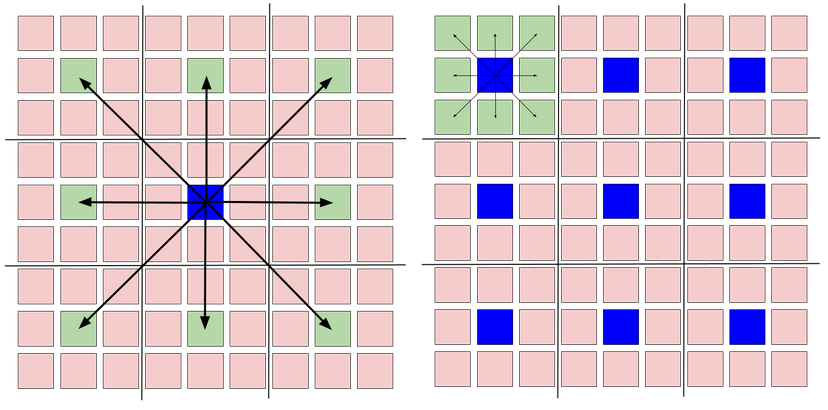
\includegraphics[width=0.95\linewidth]{panelSubdivision.png}
    \caption{Depiction of Panel Subdivision: Blue represents reference elements with known gain, green indicates elements being solved in the current iteration, and red shows elements yet to be processed. }
    \label{fig:panelSubdivision}
\end{figure}

A critical advantage of this method is the ability to parallelize the computation. After the reference alignment step, all sub-arrays can be solved in parallel. However, sub-array subdivision methods face two fundamental limitations when applied to modern phased arrays. Reference elements in the initial step may exceed practical coupling measurement distances. Additionally, elements that are close together may have saturated couplings. For the sub-array solving step, this may result in too much data sparsity for acceptable results.

These constraints motivate the development of more flexible partitioning approaches that can accommodate incomplete measurement sets and non-uniform array configurations. In many cases, this method is still the most practical way to efficiently calibrate large arrays, as the constraints mentioned can be mitigated in a variety of ways. For example, it may be possible to merge different datasets or use different power levels for each stage as long as the amplification changes between them are accounted for. In the case that these mitigation strategies are infeasible and to demonstrate that the entire calibration process can be completed in a geometry-agnostic framework, another partitioning algorithm is proposed.


%%%%%%%%%%%%%%
\subsection{Coupling Magnitude Partitioning}

\begin{figure}
    \centering
    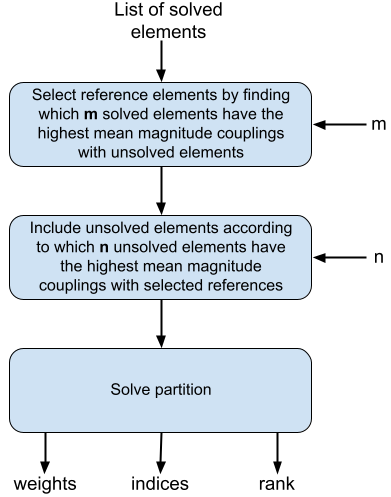
\includegraphics[width=0.75\linewidth]{Inner Scope Distcal.png}
    \caption{A flowchart depicting the partitioning process used for the coupling magnitude method. A feedback loop is utilized around this structure to determine the appropriate input parameters to this mechanism.}
    \label{fig:innerScope}
\end{figure}

\begin{figure*}
    \centering
    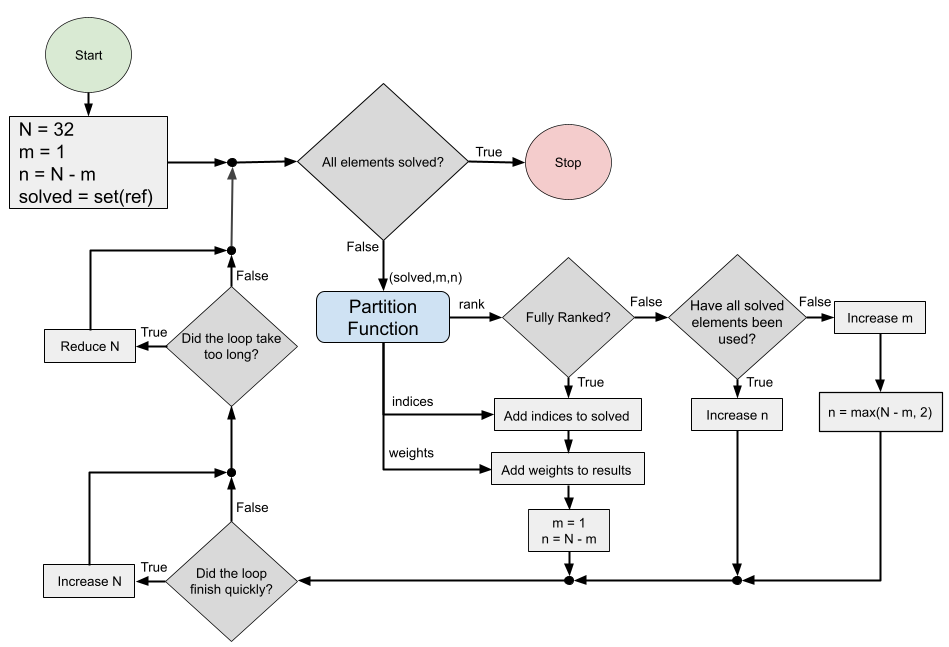
\includegraphics[width=0.9\linewidth]{Outer Scope Distcal.png}
    \caption{A flowchart depicting the feedback loop that manages the overall system while subdividing the array using magnitude partitioning.}
    \label{fig:outerScope}
\end{figure*}


 \begin{figure*}[ht]
    \centering
    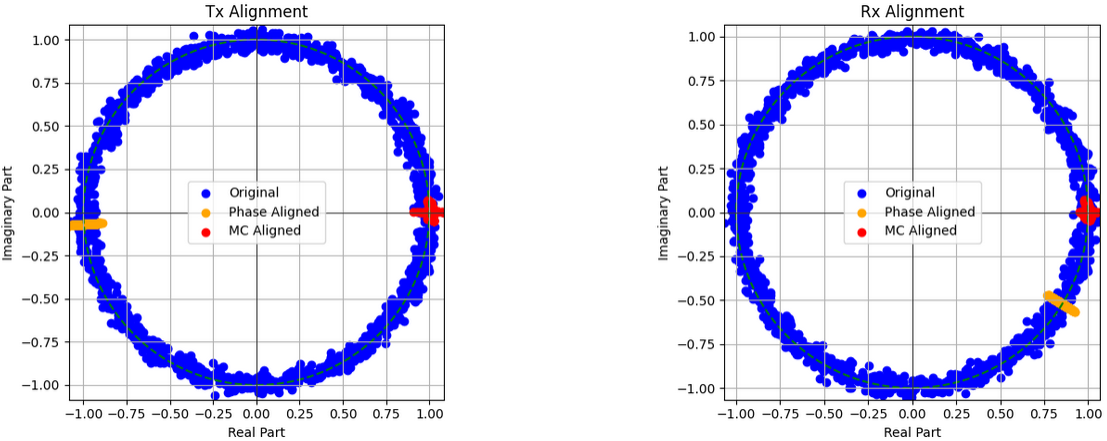
\includegraphics[width=0.95\linewidth]{agnosticSubResults-fixed.png}
    \caption{Results of magnitude partitioning applied to a dual-pol 40x40 array (800 elements, 1600 radiators, 3200 gains). Blue: The ground truth gains before calibration. Orange: After phase alignment correction is applied. Red: After phase alignment and partitioned alignment is applied. There are 1600 data points of each color in both plots; many data points overlap.}
    \label{fig:agnosticSubResult}
\end{figure*}


For most coupling datasets, elements that are close together tend to have a higher signal-to-noise ratio and are more likely to have similar connections between them. By organizing partitions according to coupling magnitude, solvable collections of elements can be identified more efficiently than by randomly selecting elements, and with higher accuracy than by selecting elements based solely on the number of connections. The steps to forming partitions with this method are as follows. First, the mean of the magnitude of the coupling values between solved elements and unsolved elements is taken. In the first loop, the "solved elements" will only be elements provided as references. The solved elements that have the highest mean magnitudes are chosen to act as references. The number of references used is set by a parameter in the function call. This operation effectively finds which solved elements are closest to the most unsolved elements. Next, a similar process is repeated where the mean is taken of couplings involved with the unsolved elements and the chosen reference elements. The unsolved elements are chosen in order of highest mean coupling magnitude. The number of unsolved elements that will be included in each pass is also set by a parameter in the function call. The elements are then formed into a partition, and the system is solved to find the weights associated with the unsolved elements. The rank of the resulting matrix is passed to the function caller along with the determined weights and their respective indices. 

If the resulting system of equations is under-ranked, detected to have a diverging inverse, or meets any other failure conditions set by the operator, the outer scope will avoid merging the results with its larger dataset and retry the function with new parameters. There are a number of parameters that can be adjusted to improve the resultant rank. For example, magnitude and angle tolerances can be increased, enabling more equations to be included in the system at the cost of precision. In practice, it is usually better to first trade execution time to improve the rank rather than sacrificing precision. By increasing the number of elements included in the subdivision, the number of connections is increased. This increases the probability of producing a fully ranked system of equations. Larger subdivisions result in much longer computation times ($O(N^4)$ complexity), but produce higher quality results and are less likely to be under-ranked. 

Increasing the subdivision size by increasing the number of reference elements produces higher quality results than increasing the number of unsolved elements. This is because including a larger number of reference elements reduces the influence of individual errors, as their effects are distributed across a broader set of equations. In addition, including more references will often result in using references that have fewer degrees of separation from the starting reference (or ideally, that include the starting reference). Conversely, increasing the number of unsolved elements per pass reduces the total number of iterations and shortens computation time. However, this approach can degrade the result quality, as each solution depends more heavily on a smaller set of references. This trade-off creates an optimization problem in which the operator must balance execution time against the accuracy requirements of the application. A diagram depicting the partitioning process is depicted in Fig.~\ref{fig:innerScope}

A practical and effective implementation explored in this work involves the use of a feedback loop to dynamically adjust the subdivision size. In this approach, the total number of elements in each partition, denoted $N$, is modulated based on timing constraints. If a partitioning iteration exceeds a predefined execution time threshold, $N$ is decreased for the subsequent pass. Conversely, if the iteration completes faster than a lower threshold, $N$ is increased. Longer time thresholds typically result in improved calibration accuracy at the expense of execution speed. To prevent excessive reductions, a lower bound is imposed on $N$.

At the start of each loop iteration, the number of reference elements, $m$, is initialized to one, and the number of unsolved elements is calculated as $n = N - m$. If the resulting system is under-ranked, $m$ is incremented to increase the proportion of references, and $n$ is updated accordingly. Assuming the execution time has stabilized within the target range, this process increases the reference density until $n$ reaches a minimum threshold, which prevents the algorithm from attempting to solve an empty or trivial system. If a satisfactory matrix rank is still not achieved when $n$ hits its lower limit, $m$ continues to increase, and $N$ is temporarily ignored. Should $m$ exceed the total number of previously solved elements, the algorithm then increases $n$ until a full-rank system is obtained. This feedback loop is depicted in Fig.~\ref{fig:outerScope}.

Although this condition was never encountered during testing, it is theoretically possible for the algorithm to attempt to include all elements in a single partition, effectively bypassing the partitioning process altogether. Prior to reaching this point, however, the computational cost would become prohibitively large. To ensure robustness, it may be advisable to implement a timeout mechanism that halts further expansion when a predefined time limit is exceeded. Upon triggering the timeout, the algorithm can either terminate gracefully or adapt by modifying other parameters. For instance, the tolerances for magnitude and phase could be incrementally relaxed until a fully ranked system is achieved. After that partition is solved, the tolerances would be reset to their start values for the next partition formation. In practice, this safeguard was not required, as none of the evaluated cases reached a state in which all previously solved elements were exhausted. The results of the coupling magnitude partitioning method applied to the Horus radar system (\cite{horuscal,horusgeneral}) configured with 800 elements are shown in Fig.~\ref{fig:agnosticSubResult}. Initially, the gains of the radiators are randomly distributed about the unit circle with uniformly distributed magnitude and phase. After phase alignment is applied, every gain is phase-aligned to the reference. After magnitude partitioning and solving with the brute force method, the gain of each element is roughly unity. There is however, a small variation in the result, which is due to the large number of elements compared to the subdivision size. The partition size used for these results was based on reasonable time constraints for the hardware available. If the application has more relaxed timing constraints, increasing execution time by adjusting the timing thresholds will generally reduce this variation if higher accuracy is required.
With these results, the array is now fully calibrated and ready for field use.
%% 
%%



%%%%%%%%%%%%%%%
%%%%%%%%%%%%%%%
\section{Conclusions}

This paper has presented a comprehensive geometry-agnostic framework for mutual coupling calibration in phased array radar systems. The proposed methodology addresses the critical limitations of traditional calibration approaches by eliminating dependence on specific array geometries while maintaining calibration accuracy. Key contributions of this work include:

\begin{itemize}
    \item Development of a generalized calibration model that accommodates both planar and non-planar array configurations through passive coupling estimation techniques.
    \item Introduction of novel phase alignment methods that outperform conventional hard-coded approaches, particularly for arrays with irregular element spacing or missing coupling data.
    \item Demonstration of an effective linearization strategy to minimize amplifier non-linearity without additional hardware.
    \item Implementation of flexible partitioning algorithms that enable calibration of large-scale arrays.
\end{itemize}

\noindent 
Experimental results demonstrate that the geometry-agnostic framework achieves comparable or superior calibration accuracy to traditional methods while offering significant advantages in operational flexibility. Many if not most of the existing mutual coupling methodologies described in the current literature can be applied using this unified computational framework. The practical implications of this research are substantial for both existing and future phased array systems. By removing geometric constraints, the new method enables calibration of conformal arrays and irregular antenna configurations, robust operation in field conditions with partial or degraded measurement data, and simplified maintenance and recalibration procedures for deployed systems. 




% BIOGRAPHIES
\FloatBarrier
\printbibliography[heading=bibintoc,title={References}]
\begin{IEEEbiography}
[{
\includegraphics[width=1in,height=1.25in,clip,keepaspectratio]{sasser.png}}]{Zachary Sasser} (Student Member, IEEE) received the B.S. degree in electrical engineering and M.S. degree in electrical and computer engineering from the University of Oklahoma, Norman, OK, USA.  Currently a graduate research assistant at the Advanced Radar Research Center (ARRC), his work focuses on all-digital radar calibration. From 2018 to 2023, he served as a production technician and software developer for the KISS Institute for Practical Robotics, developing the Wombat microcontroller and associated curriculum for Pre-K through 12th grade students to learn engineering through autonomous robotics competitions. His experience includes work at the Army Research Lab in Adelphi, Maryland. There, he gained experience with software-defined radios for beam-steering demonstrations, fabrication of military electronic systems, and phased array calibration research.
\end{IEEEbiography}


\begin{IEEEbiography}[{
\includegraphics[width=1in,height=1.25in,clip,keepaspectratio]{fulton.png}}]{Caleb Fulton}
(Senior Member, IEEE) received the B.S. and Ph.D. degrees in electrical and computer engineering from Purdue University, West Lafayette, IN, USA, in 2006 and 2011, respectively. He led the development of the Army Digital Array Radar Demonstrator at Purdue University. He is currently an Associate Professor in the School of Electrical and Computer Engineering with the Advanced Radar Research Center, The University of Oklahoma, Norman, OK, USA, where he is involved in a number of digital phased array research and development efforts for a variety of applications. His research interests include antenna design and electromagnetic analysis, digital phased array calibration and compensation for transceiver errors, calibration for high-quality polarimetric radar measurements, integration of low-complexity transceivers and high-power GaN devices, and advanced digital beamforming design considerations. He is a member of the IEEE Antennas and Propagation Society, the IEEE Aerospace and Electronics Systems Society, and the IEEE Microwave Theory and Techniques Society. He serves on the Education Committee of the latter. He received the Purdue University Eaton Alumni Award for Design Excellence in 2009 for his work on the Army Digital Array Radar Project, the Meritorious Paper Award for a summary of these efforts at the 2010 Government Microcircuit Applications and Critical Technologies Conference, and the 2015 DARPA Young Faculty Award for his ongoing digital phased-array research.
\end{IEEEbiography}

\begin{IEEEbiography}[{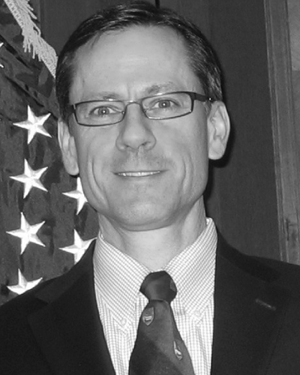
\includegraphics[width=1in,height=1.25in,clip,keepaspectratio]{yeary.png}}]{Mark Yeary}
(Fellow, IEEE) received the B.S. (Hons.), M.S., and Ph.D. degrees from the Department of Electrical Engineering, Texas A\&M University, College Station, TX, USA, in 1992, 1994, and 1999, respectively. He has served as a Principal Investigator (PI) or Co-PI on grants from NASA, NSF-ATM, NSF-DUE, NSF-ECCS, DoD-EPSCoR, NOAA-CSTAR, NOAA-NSSL, and DARPA. Since 2002, he has been with the School of Electrical and Computer Engineering, The University of Oklahoma (OU), Norman, OK, USA, where he was named the  Gallogly Chair Professor of Engineering in 2023 in OU's Gallogly College of Engineering. He is also one of the Founding Members of the Advanced Radar Research Center, OU, 2005.  His research interests include digital signal processing (DSP) as applied to customized DSP systems and instrumentation for radar systems with an emphasis on hardware prototype development and practical measurements. He served as the General Co-Chair of the IEEE Radar Conference in Oklahoma City in 2018, and he is in the planning stages to do it again in 2028.  Dr. Yeary is currently a member of the Tau Beta Pi and Eta Kappa Nu Honor societies. He is a licensed Professional Engineer.
\end{IEEEbiography}


\end{document}
